\documentclass[twoside, a4paper, 12pt]{article}

%Package Settings
\usepackage[margin=2.5cm, includefoot]{geometry}
\usepackage{setspace}
\doublespacing
\usepackage[backend=biber,authordate-trad]{biblatex-chicago}
\addbibresource{Refs.bib}
\usepackage{graphicx}
\usepackage{csquotes}
\usepackage{fancyhdr}
\usepackage{titling}
\usepackage[hidelinks]{hyperref}
\usepackage{wrapfig}
\usepackage{float}
\usepackage{caption}
\usepackage{soul}

% Page Style Stuff
\fancypagestyle{plain}{
  \fancyhf{}
  \renewcommand{\headrulewidth}{0.1pt}
  \renewcommand{\footrulewidth}{0.4pt}
  \fancyfoot[LE,RO]{\theauthor}
  \fancyfoot[C]{\thetitle}
  \fancyfoot[RE,LO]{Page \thepage}
}

% Title Formatting
\title{Greek Battle Strategy \\ And Its Victory Over Persia}

\author{Luke Hedt}
\date{\today}

\setul{}{0.2pt}

% Allows for sourcing images
\newcommand{\source}[1]{\caption*{\hfill Source: {#1}} }

% Handy Citation Notes for later:
% \footcite[200]{morris_powell_2010} %To add page numbers to citations
% \blockquote{} % If you plan to quote a huge section of Herodotus

\begin{document}

\pagenumbering{Alph}
\begin{titlepage}
    \centering
    
\includegraphics[width=0.25\textwidth]{UniLogo.png}\par\vspace{1cm}
    {\scshape\Large THE UNIVERSITY OF MELBOURNE \\
              \large ANCW20022 Ancient Greece: \\
              History and Archaeology Essay\par}
    \vspace{1.5cm}
    {\Huge \thetitle \par}
    \vfill

% Bottom of the page
    {\Large\itshape \theauthor \hspace{1em} -- \hspace{1em} 832153 \par}
    \vspace{1.5cm}
    {\Large \today}
\end{titlepage}
% Format first page correctly.
\pagestyle{plain}
\pagenumbering{arabic}

The early 5th century BC was a pivotal period in the formation of the Hellenic
identity, marking the decisive point between the period of \emph{p{\'o}leis} Greece
and the true Hellenic period. The cornerstone of this identity formation
was the defeat of Persia in the Greco-Persian Wars, beginning in 499 BC
with the Ionian Revolt. But what brought about the defeat of Persia? What tactics
were the Greeks employing in the period that brought about their victories?
This essay will attempt to address these questions, discussing how their
strategies and arms and armour were instrumental in the defeat of Persia
in the Greco-Persian Wars and
Carthage in the First Sicilian War.

\par\vspace{1em}

The Greek City States were not a cohesive unit at the outbreak of the 5th century
BC as we tend to think of them today. Rather each urban centre (the
\emph{polis}) controlled
the land around it, and considered itself a separate (and usually superior, especially
in the case of Athens)
entity to the other cities that would now be considered Greek. A person's city of
origin was usually considered more important than their `Greekness.' It was
a more prominent identifier, to be from Athens or Halicarnassus
as in the case of Herodotus, than to be Greek prior to the
Greco-Persian Wars. However, most of the Greek city states often equipped
themselves rather similarly, copying the armour style of Sparta, the most
effective fighting force in the locality.
The Greek arimes are famous for their \emph{hoplite} infanty units, heavily
armoured spear infantry with a distinctive large wooden sheild. The sheild is
the most important common component, appearing first with the
identifiable double handle in pottery art
circa 700 BC.\footnotemark
Most artistic interpretations of \emph{hoplites} tend to resemble the pottery
style in \textbf{Figure \ref{img:HopliteArcher}}, spear in the overhand
position and the sheild protecting the left-hand side of the body.
\par\vspace{1em}

\begin{wrapfigure}{R}{0.4\textwidth}
  \centering
  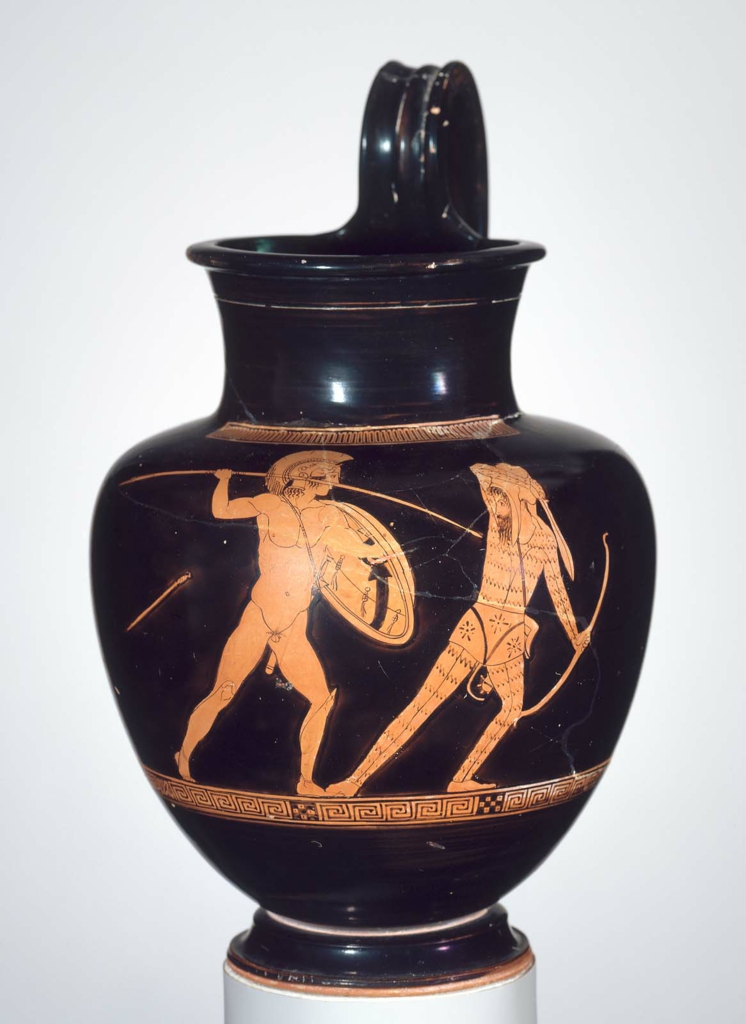
\includegraphics[width=\linewidth]{HopliteArcher.jpg}
  \captionsetup{justification=raggedleft}
  \caption{\ul{A Greek Hoplite attacking a Persian Archer, circa 450 BC.}}
  \source{\cite{MFABoston_2017_hoplite}}
  \label{img:HopliteArcher}
\end{wrapfigure}

The widely
accepted view is that these depictions are in a `heroic' pose, and not
reflective of real spear techniques. An alternative idea exists
that the technique is actually early hoplite tactics and not just a heroic
pose,\footnotemark[\value{footnote}] however the pose has several issues from
a battle perspective.
\footnotetext{\cite[57]{wees_hoplite_bronze}}
Firstly, holding the spear in such a way loses one of the main advantages of a
spear; reach. To get a balanced spear in the overhand grip, you're required
to keep over half the spear bahind your back. Not only do you lose the reach here,
but you're probably going to hit the man behind you in the head because you
can't see what you're doing. It would be far more likely that any weapon held
this way would have a counterweight on the butt of the spear, keeping it short
and balanced, but such weapons don't appear in art or archaeology. Secondly,
such a hold is very taxing on the biceps. As strong as Greek men may have been
in antiquity, it seems unlikely that anyone could be bothered holding a spear
up for the duration of a fight when you can use your elbow as a cantilever in
an under-arm grip.

\par\vspace{1em}

The Persian Empire was one of the most formidable fighting forces in the world
in the early fifth century BC, having been formed mere decades prior with
Cyrus the Great's rebellion against the Median Empire. Throughout the
Greco-Persian Wars of the fifth century, it's rather unlikely that the arms
and armourment of the Persian military evolved too much, they were after all,
the greatest army on earth, and their commander Mardonius(?) did manage
fatal overconfidence in both the battle of Marathon and Palata\^ea.

\par\vspace{1em}

In 512 BC, the Greek states were becoming restless with Persian rule. Despite
being somewhat indirect rulers of numerous Greek cities in Ionia, only requiring
a small tax from their subjects, the idea of being beholden to another nation
was insulting to the Greek cities.

\par\vspace{1em}

As a warning to all his satraps(?), Darius had to react to the Ionian
insurrection. A plan to take Athens and subjugate its leaders was formed,
and troops sailed for Greece at once from the Persian heart.

\par\vspace{1em}

A nation resisting Persian subjugation could never stand for long without
becoming the Emperor's target once again, and the Greek states were no
exception. Darius' successor Xerxes would attempt to sack Greece for its worth
and prove that Persia had military dominance in all her Empire. So once again
the Persian's sailed for Greece, landing just North of Thessaly.
Blah Blah Thermopylae.

\par\vspace{1em}

With the Spartan's defeat secured, Xerxes continued marching South for
Athens, intending to burn her, and that he did. The Athenians asked for advice
from Delphi, which was cryptic as ever.
Blah Blah burning Athens, run to the ships.

\par\vspace{1em}

With nothing but the Athenian Navy left, Persia was lead into a trap
by Thermistocles in Salamis. Big battle, many sink, much death, win Greece.

\par\vspace{1em}

Palataea and Mycale, ie Persia gets slaughtered against all odds, and
Greece gains a Hellenic identity, naming themselves around Thessaly, where
no battles were fought and nothing really happened except they got some horses
so lol?

\par\vspace{1em}

Sicilian War, Carthage takes on the Sicilian Greeks and gets its arse handed to
it.

\par\vspace{1em}

Overall Greece should have had no chance against the Persians, and the
Carthaginians probably should have been bigger baddies than they were lol.

% Bib page
\newpage
\listoffigures

\printbibliography

\end{document}
